\chapter{Background}
\label{ch:Background}

In this chapter, we present the concepts relevant to the subject of this thesis. First, we introduce the topic of MT and the type of architecture we utilize later in the work. Next, we outline the problem of ambiguity and bias in MT models.

%%%%%%%%%%%%%%%%%%%%%%%%%%%%%%%%%%%%%%%%%%%%%%%%%%%%%%%%%%%%%%%%%%%%%%%%%%%%%%%%%%%%%%%%%%%%
\section{Neural Machine Translation}
\label{sec:Background:NMT}

Machine Translation (MT) is the process of using computer technology to translate text from one natural language to another. This can be achieved using different paradigms. There are three main types of machine translation systems: Rule-based Machine Translation (RBMT), Statistical Machine Translation (SMT) and Neural Machine Translation (NMT). 

Conventional RBMT systems use pre-defined rules based on syntax, morphology and semantics, created by professional linguists. Since language is dynamic and evolves over time, these rules need frequent adaptation, which is costly. However, the key weakness of rule-based translation systems is that they require extensive lexicons and a large set of rules \parencite{SMT_book}. 

SMT systems, on the other hand, use a data-driven approach that utilizes statistical models derived from the analysis of bilingual and monolingual corpora. The quality of SMT output depends heavily on the size and quality of the corpora used to train the models. SMT’s general weakness is that it can only translate a phrase if it exists in the training dataset \parencite{SMT_book}.

Neural Machine Translation (NMT) is a subfield of SMT, which uses an artificial neural network to learn a statistical model for machine translation. Unlike traditional SMT systems, which require a pipeline of specialized components such as language model and translation model, NMT trains its statistical model end-to-end, mapping directly from an input source language to an output target language. NMT can recognize patterns in the training data to determine a context-based interpretation that can predict the likelihood of a sequence of words. Unlike SMT, NMT models are able to learn from each translation task and improve upon each subsequent translation. NMT models are more memory-efficient and also have a higher accuracy than SMT models, which makes them the appropriate choice for creating high-quality MT systems \parencite{NMT_book}.

%%%%%%%%%%%%%%%%%%%%%%%%%%%%%%%%%%%%%%%%%%%%%%%%%
\subsection{Sequence-to-Sequence Modeling}
\label{sec:Background:Seq2Seq}
The task of NMT is typically solved using Sequence-to-Sequence (Seq2Seq) modeling \parencite{seq2seq}. A Seq2Seq model has two parts: an encoder and a decoder. Both work separately and come together to form a large neural network model. This architecture has the ability to handle input and output sequences of variable length. A simplification of the architecture of NMT models can be seen in Fig. \ref{fig:seq2seq}. Firstly, each word in the input sentence is fed separately into the encoder to encode the source sentence into an internal fixed-length representation called the context vector. This context vector contains the meaning of the sentence. Secondly, the decoder decodes the fixed-length context vector and then predicts the output sequence.

The original architecture consists of a pair of Recurrent Neural Networks (RNNs) in the roles of encoder and decoder. RNNs process the input sequence token by token, which prohibits parallelization and makes the training and inference slow, especially when processing longer sequences. Also, they suffer from vanishing or exploding gradients, which is inconvenient for effective training. One solution for these problems served Long Short-Term Memory (LSTM) networks, a type of RNN that has additional memory gates to regulate the flow of information through the network better \parencite{lstm}. Despite this, using a fixed-length context vector still incurs a bottleneck in the model. To alleviate this problem, the use of attention-based architectures for neural machine translation was explored \parencite{attention}. 

The attention mechanism allows the decoder to look at the source tokens that are relevant while generating the next token. Despite all these efforts, using RNN-based encoder and decoder still forces the network to handle input sequentially, which makes it difficult to handle long-range dependencies within the input and output sequences from memory. Hence, \cite{transformer} proposed the Transformer architecture, which replaces RNNs with self-attention layers in the Encoder-Decoder network. Since in this work we make use of models based on the Transformer, next we will introduce its basic principle and components.

\begin{figure}[!htb]
  \centering
  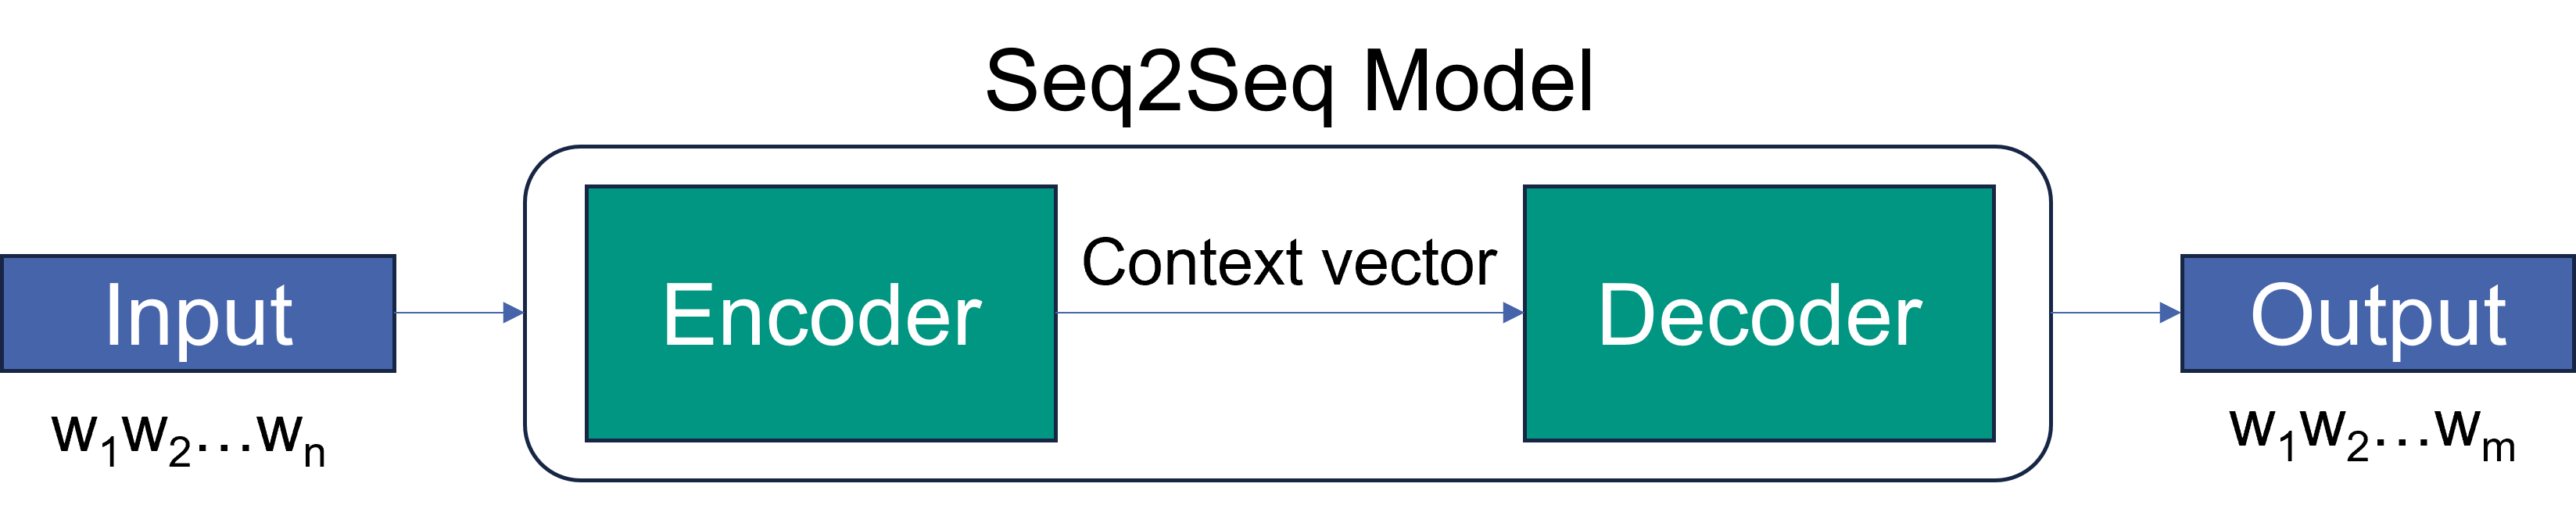
\includegraphics[scale=0.57]{figures/seq2seq.png}
  \caption{Sequence-to-Sequence Modeling}
  \label{fig:seq2seq}
\end{figure}

%%%%%%%%%%%%%%%%%%%%%%%%%%%%%%%%%%%%%%%%%%%%%%%%%
\subsection{Transformer Architecture}
\label{sec:Background:Transformer}
A Transformer is a Seq2Seq model, introduced by \citet{transformer}. An important feature of the Transformer architecture is its attention mechanism. The attention module looks at an input sequence and decides at each step which other parts of the sequence are important, differentially weighting the significance of each part of the input data. Like RNNs, Transformers are designed to handle sequential input data, such as natural language. However, unlike RNNs, Transformers can process the whole input sequence in parallel. The attention mechanism provides context for any position in the input sequence. This feature allows for more parallelization than RNNs and therefore reduces training times significantly \parencite{transformer}.

% Transformer Components
The Transformer architecture as presented in the original paper by \citet{transformer} is depicted in Fig. \ref{fig:transformer}.
The input embedding layer converts the high-dimensional input sequence into a low-dimensional sequence of vectors to capture the meaning and context.
The positional encoding preserves the sequential order of words in the input sentence and can be thought of as the distance of one word to another word in a sequence. This relative position of the words in the sequence is needed since the words are passed in parallel, as opposed to RNNs, which process them in order.
Self-attention is the weighted sum of all other words in the input sequence for each word using similarity (dot product) and SoftMax probability to focus on the most relevant parts of the input for each element. The multi-head attention repeats self-attention multiple times based on how many encoder/decoder layers there are.

There are multiple encoder and decoder layers. 
Each encoder has one multi-head self-attention, which encodes the weight of the input words to each other. 
Each decoder has one masked multi-head self-attention and one multi-head attention. The masked multi-head self-attention ensures that only words coming before a word are compared to that word, which means it only attends to preceding words in the input sequence during the decoding process. Applying a mask forces the model to ignore future words and focus only on the preceding words during the attention computation. % The mask specifically sets the attention weights to a very large negative value for the positions that correspond to future words, effectively making those weights close to zero after applying the softmax function. 
The multi-head cross-attention module in the decoder compares output tokens to input tokens.
Both the encoder and the decoder have one feed-forward layer, as well as addition and normalization of residuals at each stage after the attention layers.

The output from the decoder is a vector of length of the input tokens. This output is fed into a fully connected (linear) layer to map it to a set of output prediction and then converted into probability over possible words like multi-class classification using a SoftMax layer.


The Transformer revolutionized NMT by replacing recurrence with attention, which allowed for simultaneous computations and more effective handling of long-range dependencies. This makes it efficient on hardware like GPUs and TPUs and pushes it to be the rational choice for architecture in the realm of MT. \\


\begin{figure}[!htb]
  \centering
  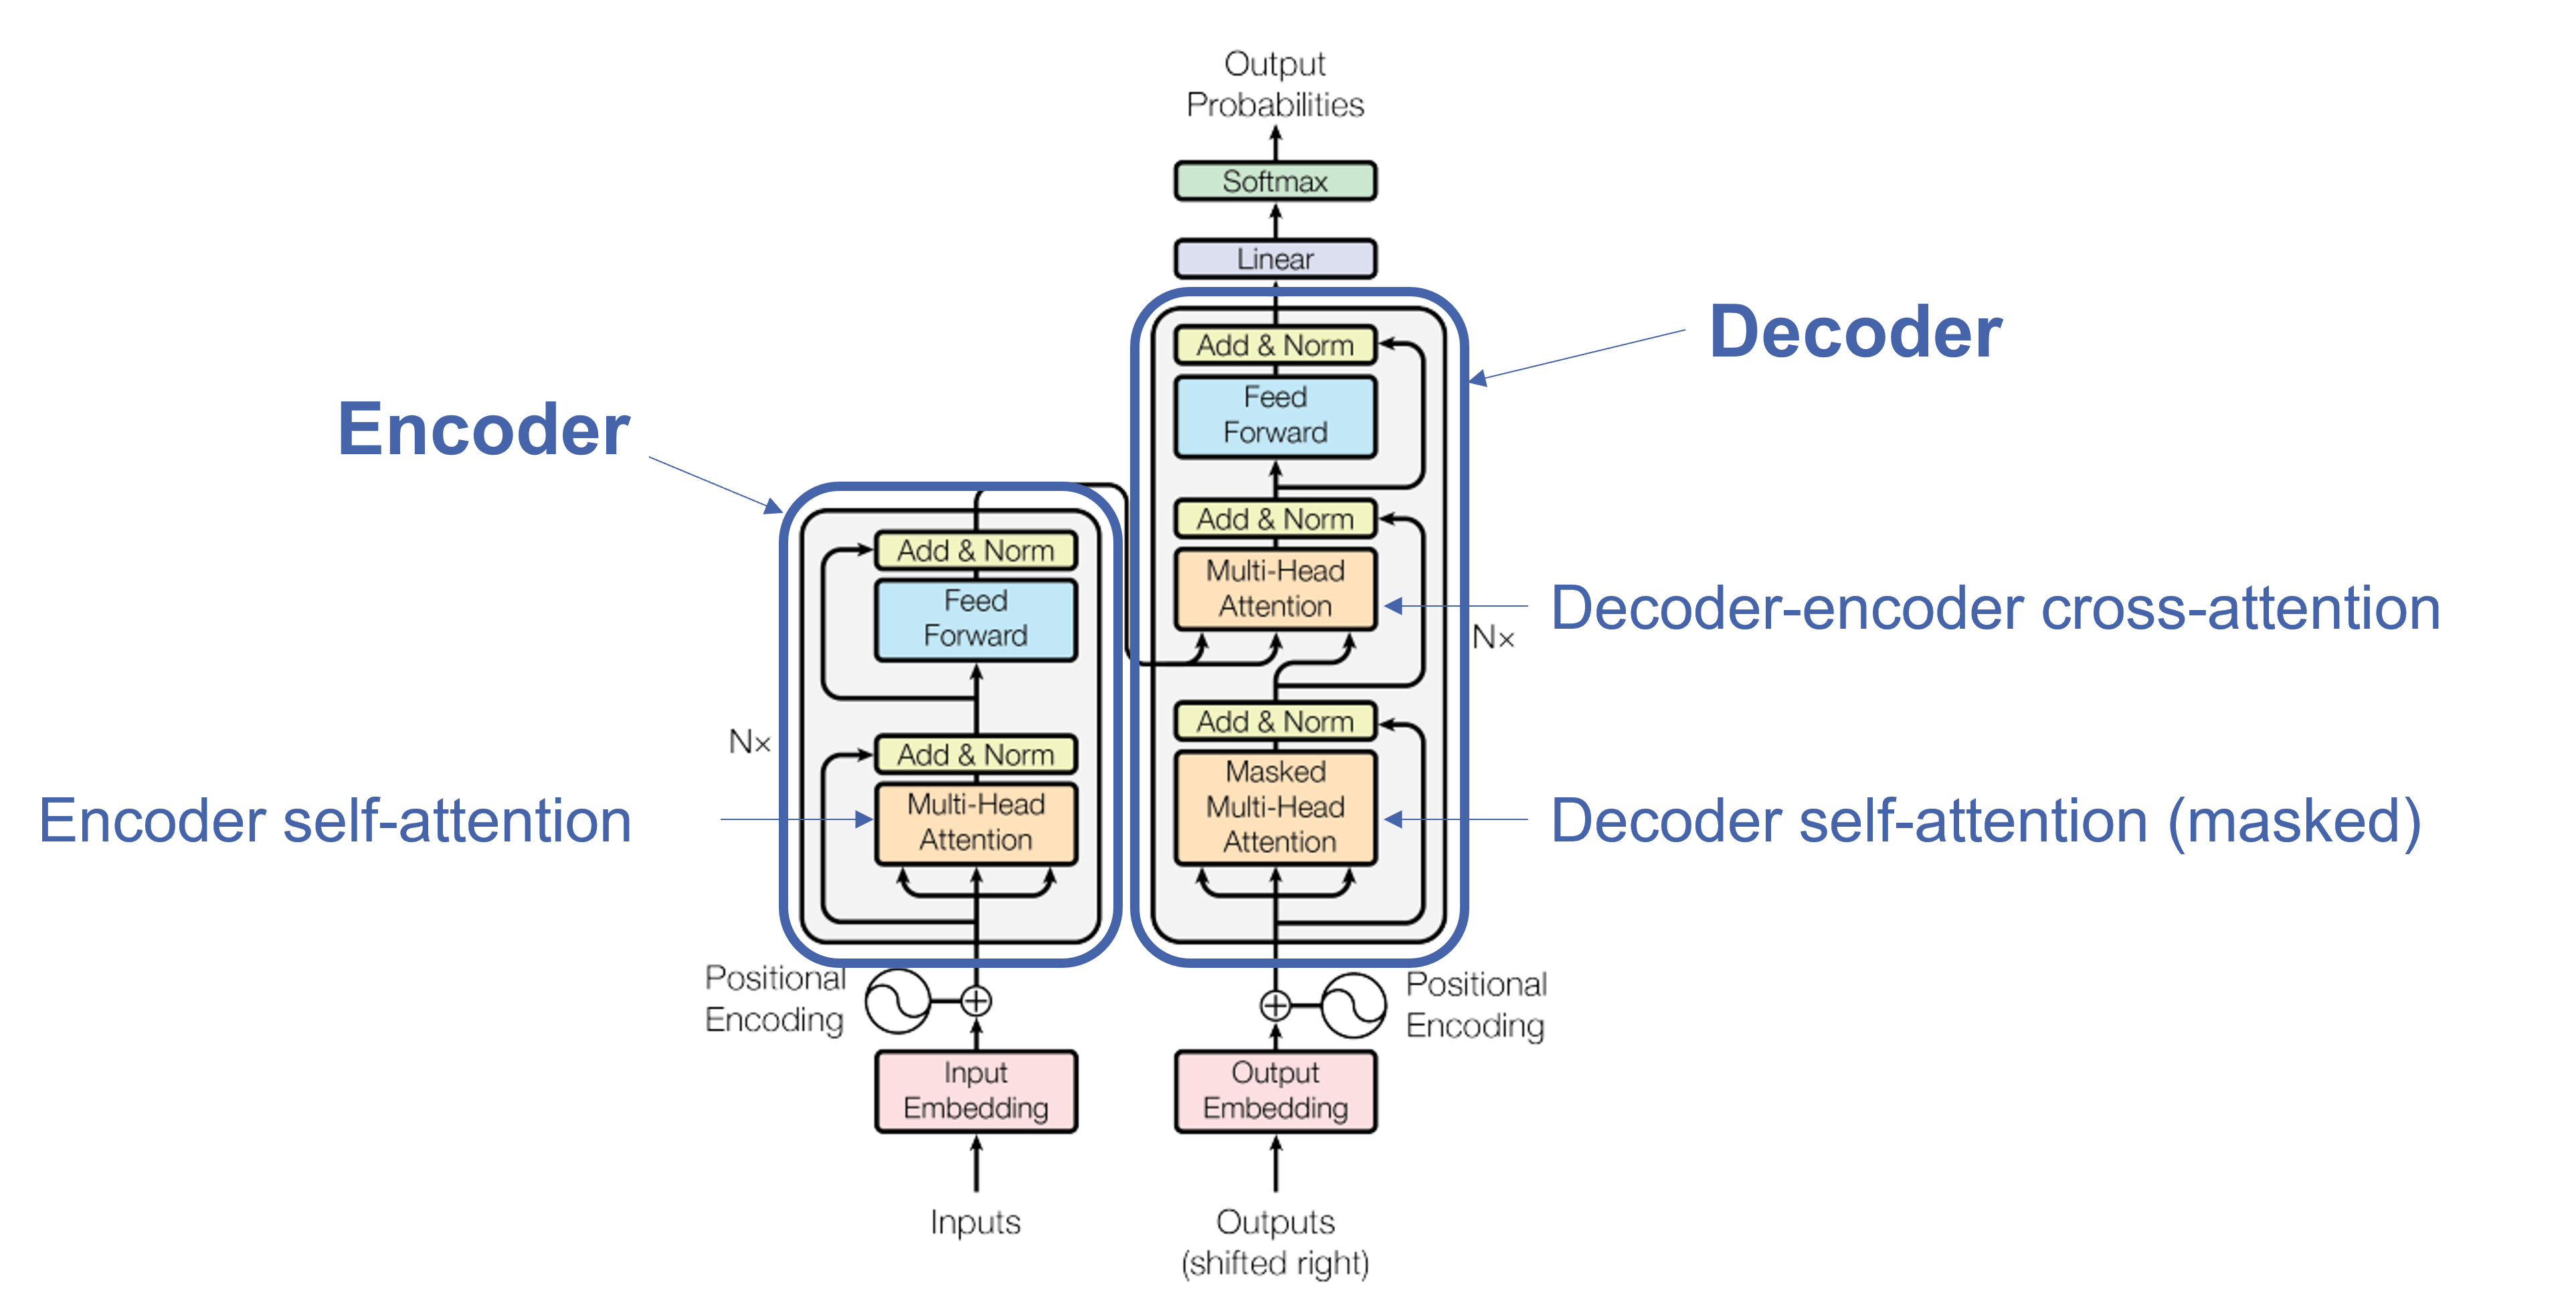
\includegraphics[scale=0.55]{figures/transformer.png}
  \caption{The Transformer Architecture}
  \label{fig:transformer}
\end{figure}

\newpage

%%%%%%%%%%%%%%%%%%%%%%%%%%%%%%%%%%%%%%%%%%%%%%%%%
\subsection{Decoding Strategies}
\label{sec:Background:Decoding}
There are multiple decoding strategies for generating translations in NMT, as presented below. 

\paragraph{Greedy search} Greedy search is the simplest decoding method. It selects the word with the highest probability as its next word. Greedy search is known to make locally optimal choices at each step, without considering the larger context. Due to this, it may not always lead to the globally optimal solution \parencite{NMT_book}.

\paragraph{Beam search} The Beam search method keeps the most likely hypotheses (beams) at each time step and eventually chooses the hypothesis that has the overall highest probability. It first predicts all possible successor words from the previous \textit{K} beams, each of which has \textit{V} possible outputs. This becomes a total of \textit{KV} paths. Out of these \textit{KV} paths, beam search ranks them by their score, keeping only the top \textit{K} paths. Beam search will always find an output sequence with higher probability than greedy search, but is not guaranteed to find the most likely output. Since Beam search is a greedy algorithm, this means that similarly to  greedy search, it makes locally optimal choices at each step with the hope that these local choices will lead to a globally optimal solution, but this is not always the case \parencite{NMT_book}.

\paragraph{Sampling} The Sampling method is non-deterministic and can generate different outputs for the same input. It selects the next word according to its probability distribution. For example, if the word “cat” has a probability of 0.6 and “dog” has a probability of 0.4, sampling might choose “dog” in some cases even though “cat” has a higher probability. Unlike Beam search, Sampling does not suffer from repetitive generation, but it may produce text that is not very coherent \parencite{NMT_book}. For this, there are a couple of different methods to modify the sampling algorithm, so that it generates more meaningful content.

\begin{itemize}
    \item Random Sampling with temperature: Random Sampling, by itself, could potentially generate a very random word by chance. Temperature is used to increase the probability of probable tokens while reducing the one that is not. Usually, the range is between 0 and 1, where 0 is the same as Greedy decoding and 1 is the same as Random Sampling.
    \item Top-K Sampling: In Top-K Sampling, the \textit{K} most likely next words are filtered and the probability mass is redistributed among only those \textit{K} next words. Only the top \textit{K} probable tokens are then considered for a generation. This technique ensures that less probable words are not chosen.
    \item Top-p (nucleus) Sampling: Instead of sampling only from the most likely K words, Top-p Sampling chooses from the smallest possible set of words whose cumulative probability exceeds the probability \textit{p}. The probability mass is then redistributed among this set of words. This way, the size of the set of words can dynamically increase and decrease according to the next word's probability distribution.
\end{itemize}

\newpage

%%%%%%%%%%%%%%%%%%%%%%%%%%%%%%%%%%%%%%%%%%%%%%%%%%%%%%%%%%%%%%%%%%%%%%%%%%%%%%%%%%%%%%%%%%%%
\section{Ambiguity and Bias in Machine Translation}
\label{sec:Background:Ambiguity_Bias}
Biases present in AI systems are an important problem stemming from cultural and historical issues present in the data from which models are learning. The developed systems in turn reinforce the present societal prejudices and old social norms, instead of mitigating them. 
It is important to understand how these biases occur in translation and to differentiate the different types of bias one may face.

Next, we will define the concepts of ambiguity and bias.

%%%%%%%%%%%%%%%%%%%%%%%%%%%%%%%%%%%%%%%%%%%%%%%%%
\subsection{Ambiguity}
\label{sec:Background:Ambiguity}
Ambiguity refers to the quality of being open to more than one interpretation, as in not having one obvious meaning. It is the type of meaning in which a phrase, statement, or resolution is not explicitly defined, making several interpretations plausible. A common aspect of ambiguity is uncertainty. In MT, ambiguity occurs when the source text leaves some essential properties unspecified, but the target language requires the property to be specified for correct translation. 

The ambiguity can be \textbf{resolvable} or \textbf{unresolvable}. It is resolvable when some semantic property required for the subject to be disambiguated can be found in the context, which defines the rest of the text available to the translation system. On the other hand, it is unresolvable, when no property necessary for disambiguation can be inferred from the context. To illustrate these two cases, we will look at two examples. When translating the sentence “She is a doctor.” from English to German, which has no gender-neutral word for “doctor”, the translation system has to choose the male (“Arzt”) or female (“Ärztin”) gender word for “doctor”. In this case, the word “doctor” is ambiguous. However, the gender is resolvable from context due to the presence of the female pronoun “she”. In contrast, the example sentence “I am a doctor.” also contains the ambiguous word “doctor”, but it is not indicated in the rest of the text whether the intended referent of “I” and “doctor” is a man or a woman. This makes the ambiguity in this case unresolvable \parencite{bias_taxonomy}.

When the ambiguity is unresolvable, the translation system cannot make an informed decision and instead applies randomness or previously acquired knowledge in choosing the translation, making an \textbf{unjustified assumption}. The assumption is unjustified because nothing actually present in the source text justifies it. In the example of “I am a doctor.” the translator typically decides for the male translation of the word “doctor”, because this case appears most often in similar contexts in its training data. Although context allows for two possible translations in German for the ambiguous word “doctor” (“Arzt” or “Ärztin”), the system will consistently prefer the male translation, which leads to a \textbf{bias} \parencite{bias_taxonomy}. 

\paragraph{Ambiguity in MT}
In this thesis, we define ambiguous words as words that have one version in the source language but multiple versions in the target language. For this purpose, we outline two different aspects of ambiguity in MT:
\begin{itemize}
    \item \textbf{General Ambiguity:} Ambiguity relating to the multiple semantic meanings of a word or phrase.
    \item \textbf{Gender Ambiguity:} Ambiguity relating to the different possible gender variations of the same word.
\end{itemize}
A single word can have both general and gender ambiguity, as well as only one or the other, or neither.

%%%%%%%%%%%%%%%%%%%%%%%%%%%%%%%%%%%%%%%%%%%%%%%%%
\subsection{Bias}
\label{sec:Background:Bias}
Bias refers to a disproportionate weight in favor of or against an idea or thing, usually in a way that is closed-minded, prejudicial, or unfair. In machine translation, it is the tendency to discriminate against certain individuals or groups in favor of others. Biases typically stem from unresolved ambiguities leading to unjustified assumptions, and can be classified as follows \parencite{bias_taxonomy}:
\begin{itemize}
    \item \textbf{Gender bias}: This type of bias occurs when there is an unresolvable ambiguity relating to the gender of people. Some commonly gender ambiguous words are professions such as doctor, teacher, cleaner. 
    \item \textbf{Number bias}: This bias presents itself when the English pronoun “you” has an unresolvable ambiguity concerning whether it refers to a single person (“du” in German) or multiple people (“ihr” in German). 
    \item \textbf{Formality bias}: This bias occurs when the English pronoun “you” has an unresolvable ambiguity concerning whether the subject is addressed formally (“Sie” in German) or informally (“du” in German). 
\end{itemize}

An MT system is biased if, while dealing with unresolvable ambiguities and deciding which unjustified assumptions to make, its decisions are not random. This means that the system makes certain unjustified assumptions more often than others. For example, if it consistently translates the occupation “doctor” as male, then the translator is biased \parencite{bias_taxonomy}.

Furthermore, biases can lead to harmful results. These can be categorized into representational and allocational harms \parencite{Savoldi_2021}. \textbf{Representational harms} detract from the representation of social groups and their identity and can be further distinguished into \textit{under-representation} and \textit{stereotyping}. Under-representation refers to the reduction of the visibility of certain social groups through language, such as producing a disproportionately low representation of women (e.g., most feminine entities in a text are misrepresented as male in translation) and not recognizing the existence of non-binary individuals (e.g., when a system does not account for gender-neutral forms). Stereotyping regards the propagation of negative generalizations of a social group, for example, belittling feminine representation to less prestigious occupations (e.g. teacher (feminine) vs. lecturer (masculine)). \textbf{Allocational harms} occur when a system allocates or withholds opportunities or resources to certain groups, for example, when a woman attempting to translate her biography by relying on an MT system requires additional energy and time to revise incorrect masculine references \parencite{Savoldi_2021}. In the long run, stereotypical assumptions and prejudices are reinforced and affect the self-esteem and behavior of members of the target group, and may also influence indirect stakeholders. 

\newpage

%%%%%%%%%%%%%%%%%%%%%%%%%%%%%%%%%%%%%%%%%%%%%%%%%
\subsection{Language Types Based on Gender}
\label{sec:Background:Language}
Currently, most of the scientific literature around biases in MT focuses on gender bias \parencite{Savoldi_2021}. In order to understand gender bias better, we need to know how it is encoded linguistically (lexical, pronominal, grammatical). There are three main language groups relating to the linguistic form of gender \parencite{Savoldi_2021}:
\begin{itemize}
    \item \textbf{Genderless languages} (e.g., Finnish, Turkish): have minimal expression of gender, relating only to lexical gender (e.g., in Finnish “sisko” (sister) and “veli” (brother)).
    \item \textbf{Notional gender languages} (e.g., English, Danish): in addition to lexical gender (mom/dad) have also pronominal gender expression (she/he, her/him).
    \item \textbf{Grammatical gender languages} (e.g., Spanish, Arabic): each noun is assigned to a class such as masculine, feminine or neutral. Grammatical gender is expressed morphosyntactically, such that several parts of speech beside the noun (e.g., verbs, determiners, adjectives) carry gender inflections.
\end{itemize}

To illustrate the difference between the different groups with an example, we look at the English sentence “He/She is a good friend.”. This sentence has no expression of gender in a genderless language like Finnish (“Hän on hyvä ystävä.”), whereas in Spanish several masculine or feminine forms are needed to express the gender (“El/Ela es un/una buen/buena amigo/amiga.”). 

